\documentclass{beamer}

\usetheme[]{Madrid}
\usepackage[symbol]{footmisc}

\title[Introduction]{Course Introduction}
\author{Will Leeson}
\date{January 19th, 2023}

\begin{document}

\begin{frame}
    \titlepage
\end{frame}

\begin{frame}
    \frametitle{Who am I?}
    \begin{columns}
        \begin{column}{0.65\linewidth}
            \begin{itemize}[<+->]
                \item Name: Will Leeson
                \item Origin: Southern Chicago Suburbs
                \item Education:
                \begin{itemize}
                    \item B.S. Computer Science (Completed)
                    \item Ph.D. Computer Science (Pursuing)
                \end{itemize} 
                \item Professional Interests
                \begin{itemize}
                    \item Software Testing and Verification
                    \item Computer Science Education
                \end{itemize}
                \item Personal Interests
                \begin{itemize}
                    \item Music and Music History
                    \item Games (Board or Video)
                    \item Cooking
                \end{itemize}
            \end{itemize}
        \end{column}
        \begin{column}{0.25\linewidth}
            \centering
            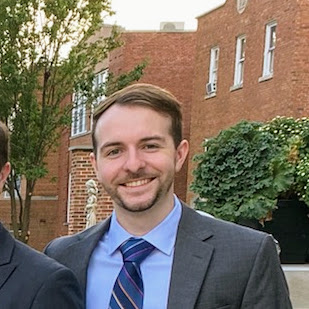
\includegraphics[width=\linewidth]{prof_pic.jpg}
        \end{column}
    
    \end{columns}
\end{frame}

\begin{frame}
    \frametitle{Course Goals}
    \begin{itemize}
        \item<1-> Understanding of the technological world
        \item<2-> Technology proficiency
        \item<3-> Critical Thinking Skills
        \item<4-> Help you succeed in future endeavours 
    \end{itemize}
\end{frame}

\begin{frame}
    \frametitle{Course Overview}
    \begin{itemize}
        \item 4 Sections
        \item 4 Homework Assignments
        \item 2 Projects
        \item 2 Exams
    \end{itemize}
\end{frame}

\begin{frame}
    \frametitle{Section 1: The Computer}
    \begin{columns}
        \begin{column}{0.45\linewidth}
            \begin{itemize}
                \item What are the components of a computer?
                \item How do computers work?
                \item The Computing revolution
                \item What is ``Big Data'' and why is it important?
            \end{itemize}
        \end{column}
        \begin{column}{0.45\linewidth}
            \centering
            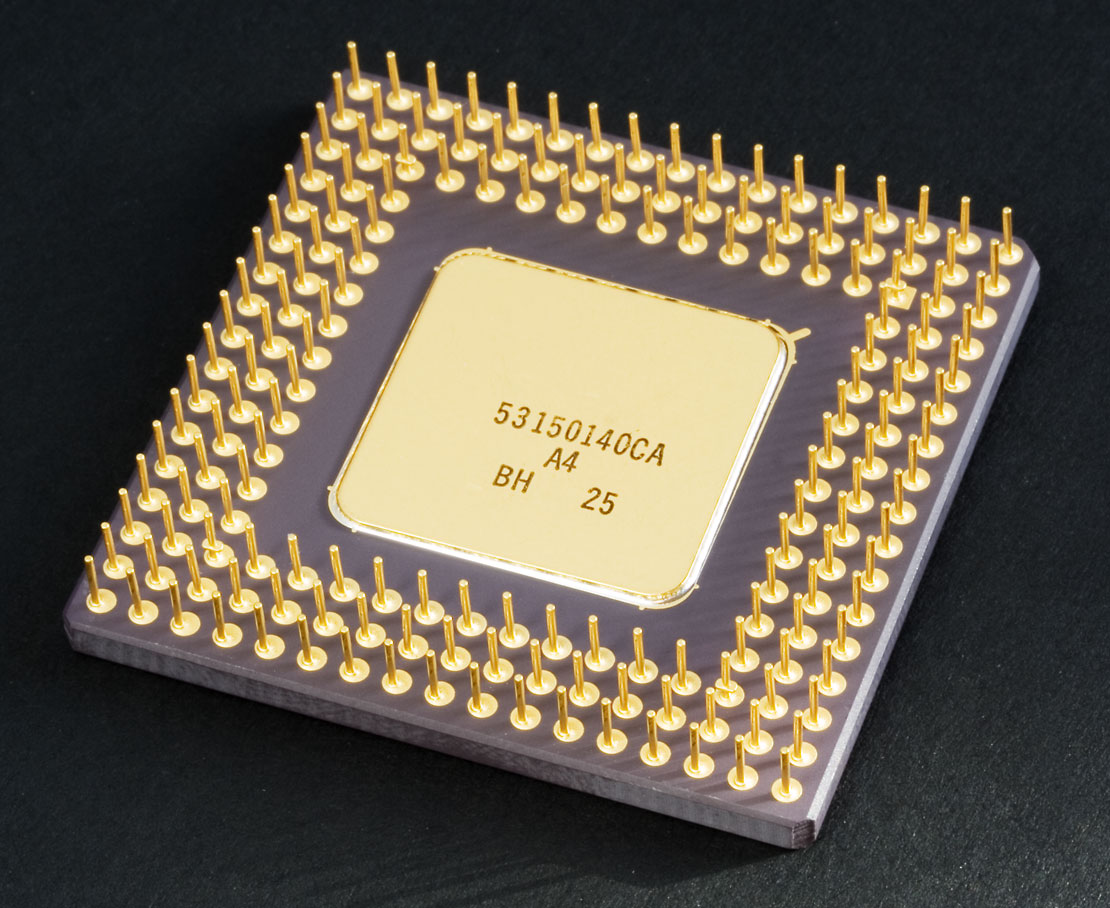
\includegraphics[width=0.5\linewidth]{cpu.jpg}
            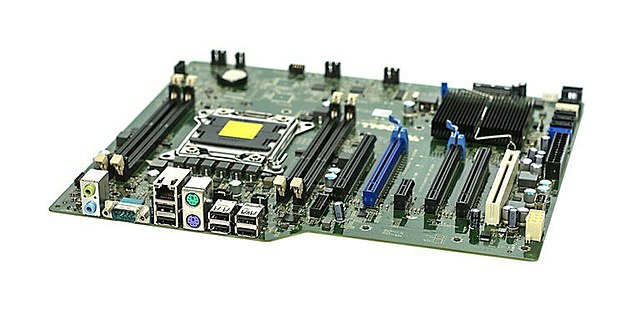
\includegraphics[width=\linewidth]{motherboard.jpg}
        \end{column}
    \end{columns}
\end{frame}

\begin{frame}
    \frametitle{Section 2: The Internet}
    \begin{columns}
        \begin{column}{0.45\linewidth}
            \begin{itemize}
                \item What is a network?
                \item The evolution of the Internet
                \item How to effectively use the Internet
            \end{itemize}
        \end{column}
        \begin{column}{0.45\linewidth}
            \centering
            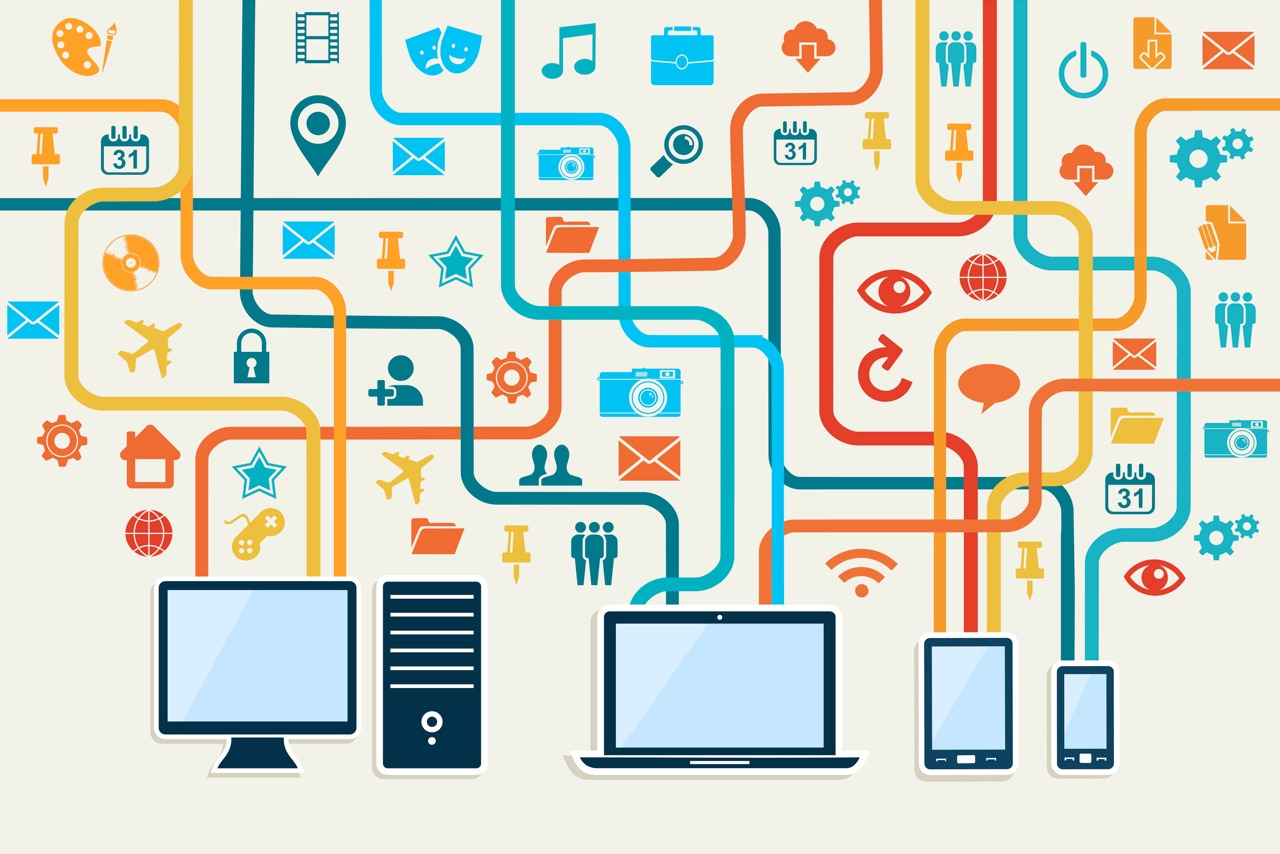
\includegraphics[width=\linewidth]{internet.jpg}
        \end{column}
    \end{columns}
\end{frame}

\begin{frame}
    \frametitle{Section 3: Programming}
    \begin{columns}
        \begin{column}{0.45\linewidth}
            \begin{itemize}
                \item<1-> How to ``think'' like a computer
                \item<2-> The basics of programming
                \item<3-> The Python programming language
            \end{itemize}
        \end{column}
        \begin{column}{0.45\linewidth}
            \centering
            \includegraphics<3>[width=\linewidth]{python.png}
        \end{column}
    \end{columns}
\end{frame}

\begin{frame}
    \frametitle{Section 4: IT in the World}
    \begin{columns}
        \begin{column}{0.45\linewidth}
            \begin{itemize}
                \item<1-> What ethical problems exist?
                \item<2-> How can I use IT solutions?
                \item<3-> TBD (What would you like to know?)
            \end{itemize}
        \end{column}
        \begin{column}{0.45\linewidth}
            \centering
            \includegraphics<3>[width=\linewidth]{python.png}
        \end{column}
    \end{columns}
\end{frame}

\begin{frame}
    \frametitle{Course Policies}

    \begin{itemize}
        \item<1-> The internet is your friend
        \begin{itemize}
            \item<2-> We don't steal from friends
            \item<3-> We borrow and give them credit
        \end{itemize}
        \item<4-> Late assignments will not be accepted
        \item<5-> I will answer all questions provided:
        \begin{itemize}
            \item<6-> You show you have thought about the problem
            \item<7-> You show you didn't give up at first signs of failure
            \item<8-> The answer to the question is not the direct answer to the problem
        \end{itemize}
    \end{itemize}
\end{frame}

\begin{frame}
    \frametitle{Grading}

    \begin{itemize}
        \item Typical Grading Scale
        \begin{itemize}
            \item A+: $>$98, A: $>$93, A-: $>$90
            \item B+: $>$88, B: $>$83, B-: $>$80
            \item C+: $>$78, C: $>$73, C-: $>$70
            \item D+: $>$68, D: $>$63, D-: $>$60
            \item F:  $<$60
        \end{itemize}
        \item Three components
        \begin{itemize}
            \item 4 Homework Assignments: 20\%
            \item 2 Projects: 40\%
            \item 2 Exams: 40\%
        \end{itemize}
    \end{itemize}
\end{frame}

\begin{frame}
    \frametitle{Other Logistics}

    \begin{itemize}
        \item Will's Office Hours: MWF 11AM-12PM or By Appointment
        \item Course Meetings: TR 5-6:15PM
        \item Course Website: https://will-leeson.github.io/CS1010/
        \begin{itemize}
            \item Includes Syllabus, Calendar, Assignments, etc.
        \end{itemize}
    \end{itemize}    
\end{frame}

\end{document}